\chapter{Android Implementation}

The workflow starts with the recording, its transcript and the target text.
Kotlin validates the inputs and segments the target. The native engine
prepares the reference features, generates target mel frames with IndicF5
and reconstructs samples with Vocos and an inverse transform. Kotlin then
joins the chunks and saves the clip for playback or export.

\section{Initialize the runtime}

\texttt{MainActivity.kt} starts the lifecycle-scoped generation job and
delegates inference to \texttt{LiteRTIndicEngine.kt}. At startup, the
wrapper copies the model assets and vocabulary to private storage when
required and invokes \texttt{nativeInitFromFile}. \texttt{jni\_bridge.cpp}
bridges model paths, PCM arrays, text, progress and telemetry.

\texttt{litert\_indic\_engine.cpp} creates a LiteRT model and interpreter
for each graph through the native C API. It sets five CPU threads and
attaches XNNPACK when available. Both interpreters reuse fixed tensor
allocations across chunks. The sampler accesses the allocated interpreter
tensors directly, avoiding the second allocation that caused problems in
the earlier signature-runner path. JNI and LiteRT still copy buffer data,
and the app holds generated waveform arrays until stitching.

\section{Acquire the reference recording and transcript}

The user enters the exact words spoken in the reference and records a
sample or selects a WAV. \texttt{AudioRecorderHelper.kt} records mono
16-bit PCM at 24 kHz. The import handler in \texttt{MainActivity.kt}
copies the file to cache and checks that it can be decoded.
\texttt{audio\_processor.cpp} reads 16-bit samples, averages channels and
converts them to floating point. The current import path assumes 24 kHz,
so recordings should already use that rate. The app checks that the engine
and inputs are ready. Transcript accuracy depends on the user's entry.

\section{Receive the target text}

The target field supplies the new words to generate. The user can type
directly or load and edit a Quick Ideas preset. The generation screen
offers 12, 16 and 24 sampling steps for Fast, Balanced and HQ,
respectively. The default is 16. When the user selects Generate,
\texttt{MainActivity.kt} captures the trimmed text and selected step count
and passes the target text to the chunker.

\section{Split longer target text into chunks}

The model has a shared window of 512 mel frames. At 24 kHz with a
256-sample hop, this corresponds to about 5.46 seconds. If the reference
occupies 356 frames, the remaining 156 represent about 1.66 seconds of
target speech per chunk. A paragraph can span multiple chunks because the
same reference is reused for every iteration.

\begin{figure}[htbp]
\centering
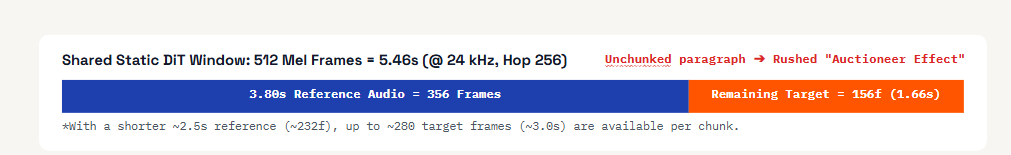
\includegraphics[width=\linewidth]{chunking-frame-budget.png}
\caption{Illustrative division of the fixed mel window between the
reference recording and target speech.}
\label{fig:chunk-budget}
\end{figure}

\texttt{MultilingualChunker.kt} protects decimal dots and common
abbreviations, then splits at sentence boundaries. It tries clause
boundaries and then word boundaries for oversized segments. It restores
protected punctuation and merges fragments shorter than 12 characters
when there is room. If it detects Devanagari, Tamil, Telugu or Kannada, it
uses a heuristic budget of 44 UTF-16 code units. The other inputs use 60.
These limits guide segmentation. The native runtime sets the final frame
allocation. For example, the input \emph{Open your books. Read the first
line.} becomes two ordered chunks, each consisting of one sentence.

\section{Extract and cache the reference mel}

After splitting the target text, the app calls \texttt{setReferenceAudio()}
once per job. \texttt{audio\_processor.cpp} measures the input RMS, raises
quiet non-negligible signals toward 0.1, applies reflection center padding
and windows each frame with a Hann window. It computes a 1,024-point FFT
every 256 samples, applies 100 mel filters and takes the log after applying
a small floor. \texttt{litert\_indic\_engine.cpp} caches the mel, reference
frame count and transcript for every chunk in the job.

\section{Allocate target duration and build model inputs}

Let $R$ be the cached reference frame count, $B_r$ the reference transcript
length in bytes and $B_g$ the target length in bytes. The inference engine
estimates a requested target length and limits it to the remaining window.
\[
G_0=\max\left(80,\left\lfloor
1.15 R\frac{\max(1,B_g)}{\max(1,B_r)}
\right\rfloor+10\right),\qquad G=\min(512-R,G_0).
\]
The requested 80-frame minimum applies before the cap. A long reference can
therefore leave fewer than 80 frames for target speech.

The engine copies the reference mel into the leading rows of a zero-filled
conditioning tensor. It combines the transcript and target chunk and
appends terminal punctuation when the native punctuation rule calls for
it. \texttt{indic\_tokenizer.cpp} maps the text to vocabulary IDs, truncates
or pads to 128 positions and uses $-1$ for padding and unknown entries.
The text-token limit applies independently of the acoustic window.

\section{Generate acoustic features with IndicF5}

\texttt{euler\_sampler.cpp} initializes the latent with Gaussian noise
and uses seed $42+$ the zero-based chunk index. Each step runs IndicF5 with
the reference mel and text, then runs the same graph with zero conditioning
and pad-only tokens. With $v_c$ and $v_u$ as the conditioned and
unconditioned predictions, the update is
\[
v=v_c+2.0(v_c-v_u),\qquad
x_{i+1}=\operatorname{clip}(x_i+(t_{i+1}-t_i)v,-4.5,4.5).
\]
For $N$ steps, the current cosine-sway coefficient of $-1$ gives
$t_i=1-\cos(\pi i/(2N))$. At the default 16 steps, each chunk makes 32
DiT invocations. The app reports chunk and sampling progress.
Cancellation is cooperative and takes effect when execution reaches a
sampling or chunk checkpoint.

\section{Reconstruct and join the waveform}

\texttt{litert\_indic\_engine.cpp} restores the reference mel prefix and
transposes the generated mel for Vocos. The decoder produces 513 complex
frequency bins per frame as real and imaginary planes.
\texttt{audio\_processor.cpp} performs the inverse transform with KissFFT,
overlaps Hann-windowed frames, normalizes by the window envelope and
removes center padding. The engine slices the region allocated to the
target after the reference section. When the cropped peak is at least
0.03, the engine scales it to 0.95.

\texttt{WaveformStitcher.kt} trims quiet edges with an amplitude threshold
of 0.012. It retains 25 ms at the leading and intermediate trailing edges
and 120 ms at the final trailing edge. It applies 5 ms raised-cosine fades,
inserts 30 ms of silence between chunks, appends 450 ms of trailing silence
and peak-normalizes the assembled waveform to 0.95. The app fades each
chunk individually and concatenates them in order.

\section{Save, play, download and share}

\texttt{GenerationHistoryManager.kt} writes one 24 kHz mono 16-bit PCM WAV
to app-private storage and updates the local clip library.
\texttt{AudioExporter.kt} uses MediaStore for Downloads on Android 10 and
later, with a legacy file path on earlier versions. The share action in
\texttt{MainActivity.kt} opens the Android share sheet with an
\texttt{audio/wav} content URI and temporary read access. The current
inference loop skips empty chunks. If some chunks succeed, a file can
therefore contain only part of the requested text.

\section{Worked example: trace one chunk to the WAV}
\label{sec:worked-example}

The first chunk in the two-sentence example is \emph{Open your books.}
It contains 16 ASCII bytes. For this trace, assume a 40-byte reference
transcript and 356 cached reference mel frames.

\begin{enumerate}[nosep]
  \item \textbf{Allocate the window.} The duration heuristic requests
        $\lfloor 1.15\times356\times16/40\rfloor+10=173$ target frames.
        The shared 512-frame window caps this at $512-356=156$ frames,
        a nominal target budget of about 1.66 seconds.
  \item \textbf{Prepare and sample.} The engine copies the reference mel into
        the first 356 rows of the conditioning tensor and encodes the
        transcript and target together. With seed 42 for chunk index zero,
        it takes 16 Euler steps. The conditioned and unconditioned passes
        make 32 IndicF5 calls in total.
  \item \textbf{Decode and crop.} One Vocos invocation decodes the sampled
        mel. After inverse reconstruction and center-padding removal, the
        512-frame output spans $511\times256=130{,}816$ samples. The native
        crop starts at $356\times256=91{,}136$ and ends at the available
        length, yielding 39,680 target samples (about 1.65 seconds) before
        stitching.
  \item \textbf{Join and save.} The stitcher trims and fades the chunk,
        inserts a 30 ms gap before the second chunk, and adds 450 ms of
        trailing silence after the last chunk. Kotlin writes one 24 kHz
        mono 16-bit PCM WAV. Its final duration depends on the retained
        samples from both chunks and the inserted silence.
\end{enumerate}
